\documentclass{article}

% Set Language to english
\usepackage[english]{babel}

% Set page size and margins
\usepackage[a4paper,top=2cm,bottom=2cm,left=3cm,right=3cm,marginparwidth=1.75cm]{geometry}

% Useful packages
\usepackage{amsmath}
\usepackage{graphicx}
\usepackage{stackengine}
\usepackage{array}
\usepackage{tabularx}
\usepackage{makecell}
\usepackage{float}

\usepackage[colorlinks=true, allcolors=blue]{hyperref}
\usepackage{setspace}
\usepackage[round, comma]{natbib}
\usepackage{ragged2e}

\newcommand{\approxsim}{\mathrel{\stackon[1pt]{\stackunder[1pt]{\sim}{\cdot}}{\cdot}}} % create symbol for approximately distributed




\begin{document}

% TITLE PAGE

\begin{titlepage}
\begin{center}

\Large 

Methodology and Statistics for the Behavioural, Biomedical and Social Sciences \vspace{0.5cm}

Utrecht University
    
\vspace{0.5cm}
      
\rule{\textwidth}{1.5pt}
\LARGE
\textbf{Research Report}

\vspace{0.25cm}
\textbf{Refining Relational Event Models: Bayesian Penalization and Variable Selection in REMs} \\
\vspace{0.25cm}
\rule{\textwidth}{1.5pt}

\vfill

\Large
\textbf{Jonathan Koop} \vskip 0.05in
\normalsize
4972155 \vskip 0.05in
j.koop@uu.nl

      

\vfill

\normalsize

Supervisors: \vskip 0.05in
\large
Mahdi Shafiee Kamalabad 

Sara van Erp \vskip 0.05in

\vfill

\normalsize
Ethical Approval Case No.: 24-2053, 24-2054, 24-2057\vskip 0.05in
Candidate Journal: \textit{Social Networks} \vskip 0.05in
Word Count: 2,498

\end{center}
\end{titlepage}


% MAIN

\begin{spacing}{2}
\begin{justify}

\section{Introduction}

In the age of big data, the availability of detailed records of social interactions over time—referred to as relational event history (REH) data—offers unprecedented opportunities to investigate the dynamics of complex networks. In contexts ranging from animal behavior \citep{Tranmer2015} to acts of violence within criminal networks \citep{Niezink2022}, REH data prompts researchers to examine the factors that drive these relational events. To achieve that, relational event models (REMs) have emerged as the gold standard \citep{Butts2008}, as they account for the data's dynamic nature.

Due to scarce theoretical literature on the drivers of relational events \citep{Karimova2023}, choosing appropriate variables from the multitude of potential predictors poses a significant challenge to applied researchers utilizing REMs. Many node or edge attributes, termed exogenous variables (e.g., age or gender), can be used to explain the rate of interactions among actors \citep{MeijerinkBosman2022}. Specific to REH data is the existence of endogenous variables summarizing characteristics of previous relational events at a specific time point. One of these is inertia, reflecting the frequency of prior interactions (with the same direction) between the same actors \citep{Leenders2016}. Numerous endogenous variables, in addition to inertia, complicate the identification of key variables \citep{Butts2008}, resulting in a large number of potential predictors to include in a model.

For efficiently identifying a model and avoiding overfitting, different regularized regression techniques were introduced for linear models \citep{Hastie2015} promising the selection of important predictors: In classical frameworks, techniques such as Ridge regression \citep[$\ell_2$ norm;][]{Hoerl1970} and LASSO  \citep[$\ell_1$ norm;][]{Tibshirani1996} are prominently applied. Their Bayesian counterpart, Bayesian regularization, has been shown to perform equally or better by incorporating shrinkage through zero-centered prior distributions, providing more reliable parameter uncertainty estimates and allowing simultaneous estimation of model and penalty parameters \citep{vanErp2019}. \par

In REMs, regularization has gained surprisingly little attention. Recently, \citet{Karimova2023} applied Bayesian regularization on multinomial Probit models to select predictors for REH data.  They conclude that it can effectively reduce Type-I errors while maintaining high predictive performance. A comparison of these results to an approximate Bayesian regularization procedure found both approaches to perform similarly \citep{Karimova2024}.\par

What remains missing is a systematic investigation of Bayesian regularization in REMs across varying sample and effect sizes, providing applied researchers with guidance on selecting adequate methods for their data. Therefore, the thesis project addresses the research question of \textit{How can Bayesian regularization and variable selection improve the identification of effects in relational event models?}

To address this question, the overarching aim of the project is the systematic application of Bayesian regularization to REMs. As a preliminary step, this report evaluates the performance of approximate Bayesian regularization (ABR) against methods relying solely on maximum likelihood estimation (MLE), comparing variable selection and predictive performance across multiple settings.

\section{Methodology}

\subsection{Statistical Underpinnings}

\subsubsection{The Relational Event Model}

REMs provide a flexible framework for analyzing fine-grained dynamic interaction data, allowing for the estimation of the likelihood of relational events over time \citep{Butts2008}. They build on the assumption that time intervals between events follow an exponential distribution, where the rate parameter $\lambda$ varies as a function of covariates. At any given time $t$, the overall event rate is expressed as $\lambda_t' = \sum_{s,r} \lambda^{\text{REM}}(s,r,t)$, with $\lambda^{\text{REM}}(s,r,t)$ representing the rate of an event from sender $s$ to receiver $r$. The summation includes all pairs within the riskset $\mathcal{R}_t$ summarizing every plausible combination of senders and receivers at time $t$. Consequently, the time intervals between events are assumed to be distributed as
\begin{equation}
    \Delta t \sim \text{Exponential}(\lambda_t') \label{eq:rem_exp}
\end{equation}

The specific event rates are determined through a log-linear model of covariates such that
\begin{equation}
    \log \lambda^{\text{REM}}(s,r,t) = X_{s,r}(t)'\beta, \label{eq:rem_equation}
\end{equation}

where $X_{s,r}(t)$ denotes the covariate vector, including both exogenous and endogenous statistics, and $\beta$ represents the vector of regression coefficients. The probability of a given event, for which sender $s'$ interacts with receiver $r'$, is defined as a multinomial probability, with probability mass function
\begin{equation}
p((s, r) = (s', r') | \mathcal{A}_t) = \frac{\lambda^{\text{REM}}(s', r', t)}{\sum_{s, r} \lambda^{\text{REM}}(s, r, t)}, \label{eq:rem_multinomial}
\end{equation}

where $\mathcal{A}_t$ represents the relational event history up to time $t$. This formulation allows REMs to account for the full interaction history, providing a framework for dynamic relational processes.

With the wide availability of both exogenous and endogenous variables \citep{Butts2008}, comes the risk of overfitting and overcomplicating the model's interpretability by including too many predictors and their interaction effects. Thus, identifying a sparse model including the relevant predictors while excluding spurious effects is crucial.

\subsubsection{Approximate Bayesian Regularization}

In identifying such a model, penalized regression techniques, specifically LASSO and Ridge regression, enjoy widespread popularity \citep{Hoerl1970, Tibshirani1996}. Given drawbacks such as the LASSO’s underestimation of standard errors \citep{Casella2010} and computational challenges, Bayesian regularization has gained recent popularity. Applying Bayes' theorem, coefficients are shrunken, with a posterior distribution influenced by the likelihood function and a prior distribution centered around zero. Markov Chain Monte Carlo (MCMC) sampling consequently allows simultaneously estimating coefficients and penalty parameters \citep{vanErp2019}. 

Beneficial to Bayesian regularization is particularly its ability to include several prior distributions, going beyond Bayesian equivalents to LASSO and Ridge regression with Laplace and Normal prior distributions, respectively \citep{Park2008, Loesgen1990}. Particularly, nonconcave horseshoe priors \citep{Carvalho2010} have demonstrated strong performance \citep{vanErp2019}, as their shape — characterized by a high probability mass near zero combined with heavy tails — enables strong shrinkage of weak coefficients towards zero while maintaining strong effects of larger coefficients. 

Despite its advantages, Bayesian MCMC algorithms can be computationally slow, limiting their practical use \citep{Karimova2024}. To address this disadvantage, \citet{Karimova2024} introduced Approximate Bayesian Regularization (ABR) approximating the likelihood function of $\beta$ by a Normal distribution centered around the MLE estimates $\hat{\beta}_{MLE}$ with the error covariance matrix $\hat{\Sigma}_{\beta}$ as covariance matrix:

\begin{equation}
    p(D \mid X, \beta) \sim \mathcal{N}(\beta \mid \hat{\beta}_{\text{MLE}}, \hat{\Sigma}_{\beta})
    \label{eq:approximation_likelihood}
\end{equation}

Combining this with a shrinkage prior $p_{Bayes}(\beta | \lambda) \, p(\lambda)$ leads to the following posterior distribution:

\begin{equation}
    \hat{p}_{Bayes}(\beta, \lambda | D, X) \propto N(\beta | \hat{\beta}_{MLE}, \hat{\Sigma}_{\beta}) \, p_{Bayes}(\beta | \lambda) \, p(\lambda) \text{.}
    \label{eq:bayesian_inference}
\end{equation}

Applying this here, a REM is estimated using MLE to derive unregularized estimates $\hat{\beta}_{MLE}$ and their associated error covariance matrix $\hat{\Sigma}_{\beta}$. These serve as the distribution parameters for a Normal distribution to approximate the likelihood function of $\beta$. Regularization is consequently introduced by combining this Normal approximation with a prior distribution centered around zero. By MCMC sampling a posterior distribution is obtained.

In practice, Bayesian regularization, whether using the exact likelihood function or this approximation, has been shown to enhance the predictive performance of REMs. Applying exact Bayesian regularization, \citet{Karimova2023} evaluated the performance of different models by examining the proportion of observed events that fell within the top 5\%, 10\%, and 20\% most probable events predicted by the models. Regularized Bayesian REMs with Ridge, LASSO, and Horseshoe priors were found to perform comparably to standard MLE-based REMs when predicting in-sample observations from voice loops during the Apollo mission, i.e., events used for training the REM. Moreover, they observed the regularized models to outperform the former with regards to out-of-sample observations, indicating that regularization may indeed reduce overfitting.

Demonstrating the use of ABR for REMs, \citet{Karimova2024} observed ABR with Ridge, LASSO, and Horseshoe priors to perform similarly to exact Bayesian methods. An application on Apollo 13 voice loop data demonstrated similar in-sample predictive performance and slightly lower out-of-sample performance compared to the exact approach.

While encouraging, the performance of ABR in REMs across different numbers of events $M$ and effect types remains to be systematically explored.

\subsection{Simulation Study}

\subsubsection{Data Generation and Conditions}

To evaluate the performance of ABR in selecting variables and making predictions within REMs, a simulation study is conducted comparing it to standard MLE procedures. Consequently, REH data is generated with the event rate being explained by the inclusion of three endogenous effects identified on Apollo-13 data \citep{ShafieeKamalabad2023} and six exogenous variables, three of which were continuous ($Z_1$, $Z_2$ and $Z_3$) and three binary ($Z_4$, $Z_5$ and $Z_6$). Effect sizes of the natural logarithms of 1.22 for weak, 1.86 for moderate, and 3.00 for strong effects were assigned to one variable each following the conventions used in Cox proportional hazard which can be applied to REMs \citep{Olivier2017, Schecter2020}. The remaining 29 endogenous statistics for directed relational events in the \texttt{remstats} R package \citep{remstats} and an additional 10 exogenous variables were specified to have no effect, leading to the data generating model
\begin{equation}
\begin{aligned}
    \log \lambda^{\text{REM}}(s,r,t) = & -8 + 0.7 \, \text{IndegreeSender}(s,r,t) + 0.15 \, \text{Reciprocity}(s,r,t) \\
    & - 0.45 \, \text{OutdegreeReceiver}(s,r,t) + \log(1.22) \, \text{Min}(Z_1) + \log(1.22) \, \text{Max}(Z_1) \\
    & + \log(1.86) \, \text{Min}(Z_2) + \log(1.86) \, \text{Max}(Z_2) \\
    & + \log(3.00) \, \text{Min}(Z_3) + \log(3.00) \, \text{Max}(Z_3) \\
    & + \log(1.22) \, \text{Same}(Z_4) + \log(1.86) \, \text{Same}(Z_5) \\
    & + \log(3.00) \, \text{Same}(Z_6) \text{.}
\end{aligned}
\label{eq:rem_model}
\end{equation}

In accordance with \citet{Lakdawala2024}, REH data was generated by iteratively computing $\lambda^{REM}(s,r,t)$, drawing the time interval $\Delta t$ from distribution \eqref{eq:rem_exp} and sampling the next dyad from distribution \eqref{eq:rem_multinomial}. Data were generated with $M = 3200$ events and $N=50$ potential actors of which all 2450 dyads were in the riskset $\mathcal{R}_t$ at all $t$. Due to computational limitations, 50 of these datasets were generated.

To assess the effect of the number of events $M$ on variable selection performance, each dataset is subsetted to include the first 100, 200, 400, 800, 1600, and finally all 3200 events, resulting in 300 datasets in total.

\subsubsection{Evaluation of the Performance}

To evaluate the performance in discovering the true data-generating model, three models were estimated: A standard REM relying simply on the MLE estimates, a model resulting from ABR with a Ridge prior, and an ABR model with a Horseshoe prior. As selection criterion for MLE estimates, univariate selection at $\alpha = 0.05$ (i.e., variables with statistically significant effects in the full model) served as a rather naive selection criterion. For the two models resulting from ABR, the 95\% highest density interval criterion (HDI; i.e., choosing variables with intervals that exclude zero) was applied.

For these criteria true discovery rates were computed, averaging over the three endogenous effects, and the three effect sizes for exogenous effects. These rates capture the proportion of variables with truly nonzero effects being selected. False discovery rates - capturing the proportion of variable with no truly nonzero effect being selected - were calculated separately for endogenous and exogenous effects. Moreover, the capacity to recover the true parameters was assessed by analyzing the estimates' bias and variance. Bias was quantified as the average deviation of the estimates from the true effects over the 50 iterations, and variance as the variance of this deviation across replications. To assess predictive performance of the three models, both, in-sample and out-of-sample metrics were used. Event rates were calculated at each $t$ and the proportion of cases in which the actual event is included in the 5\%, 10\%, and 20\% highest probability events were evaluated. For in-sample performance, this was applied to all events that were used to train the REM. For out-of-sample performance the next 500 out-of-sample events were evaluated. Thus, there was no assessment of the model trained on all 3200 events since no events were generated thereafter. The models, the applied selection criteria, selection evaluation, and predictive performance measures are displayed in Table \ref{tab:model_comparison}.


\begin{table}[h]
\centering
\renewcommand{\arraystretch}{1.3} % Set row spacing
\caption{Overview of variable selection criteria, selection evaluation, and predictive performance measures used in the three models: Maximum Likelihood Estimation (MLE), Approximate Bayesian Regularization with Ridge prior (ABR Ridge), and Approximate Bayesian Regularization with Horseshoe prior (ABR HS). HDI abbreviates Highest Density Interval.}
\begin{tabularx}{\textwidth}{p{4.2cm} X X X} \hline
\textbf{Model} & \textbf{MLE} & \textbf{ABR (Ridge)} & \textbf{ABR (HS)} \\ \hline
\textbf{Applied Selection Criterion} & Univariate Selection ($\alpha=0.05$) & 95\% HDI & 95\% HDI \\ \hline
\noalign{\vskip 0.5em} % Add vertical space
\textbf{Selection Evaluation} & \multicolumn{3}{l}{\makecell[l]{True and False Discovery Rates}} \\ \hline
\noalign{\vskip 0.5em} % Add vertical space
\textbf{Predictive Performance Measure} & \multicolumn{3}{l}{\makecell[l]{Proportion of Events in Which Observed Event Falls in Top 5\%,\\ 10\%, and 20\% Most Probable Events (In-Sample and Out-Of-\\Sample)}} \\ \hline
\end{tabularx}
\label{tab:model_comparison}
\end{table}

Analyses were conducted in \textit{R} 4.4.0 \citep{R}, using \texttt{remify} \citep{remify}, \texttt{remstats} \citep{remstats}, \texttt{remstimate} \citep{remstimate}, and \texttt{shrinkem} \citep{Karimova2024}. The code is available at \url{https://github.com/jonathankoop/ResearchReport}.

\section{Preliminary Results}

\begin{figure}[H]
    \centering
    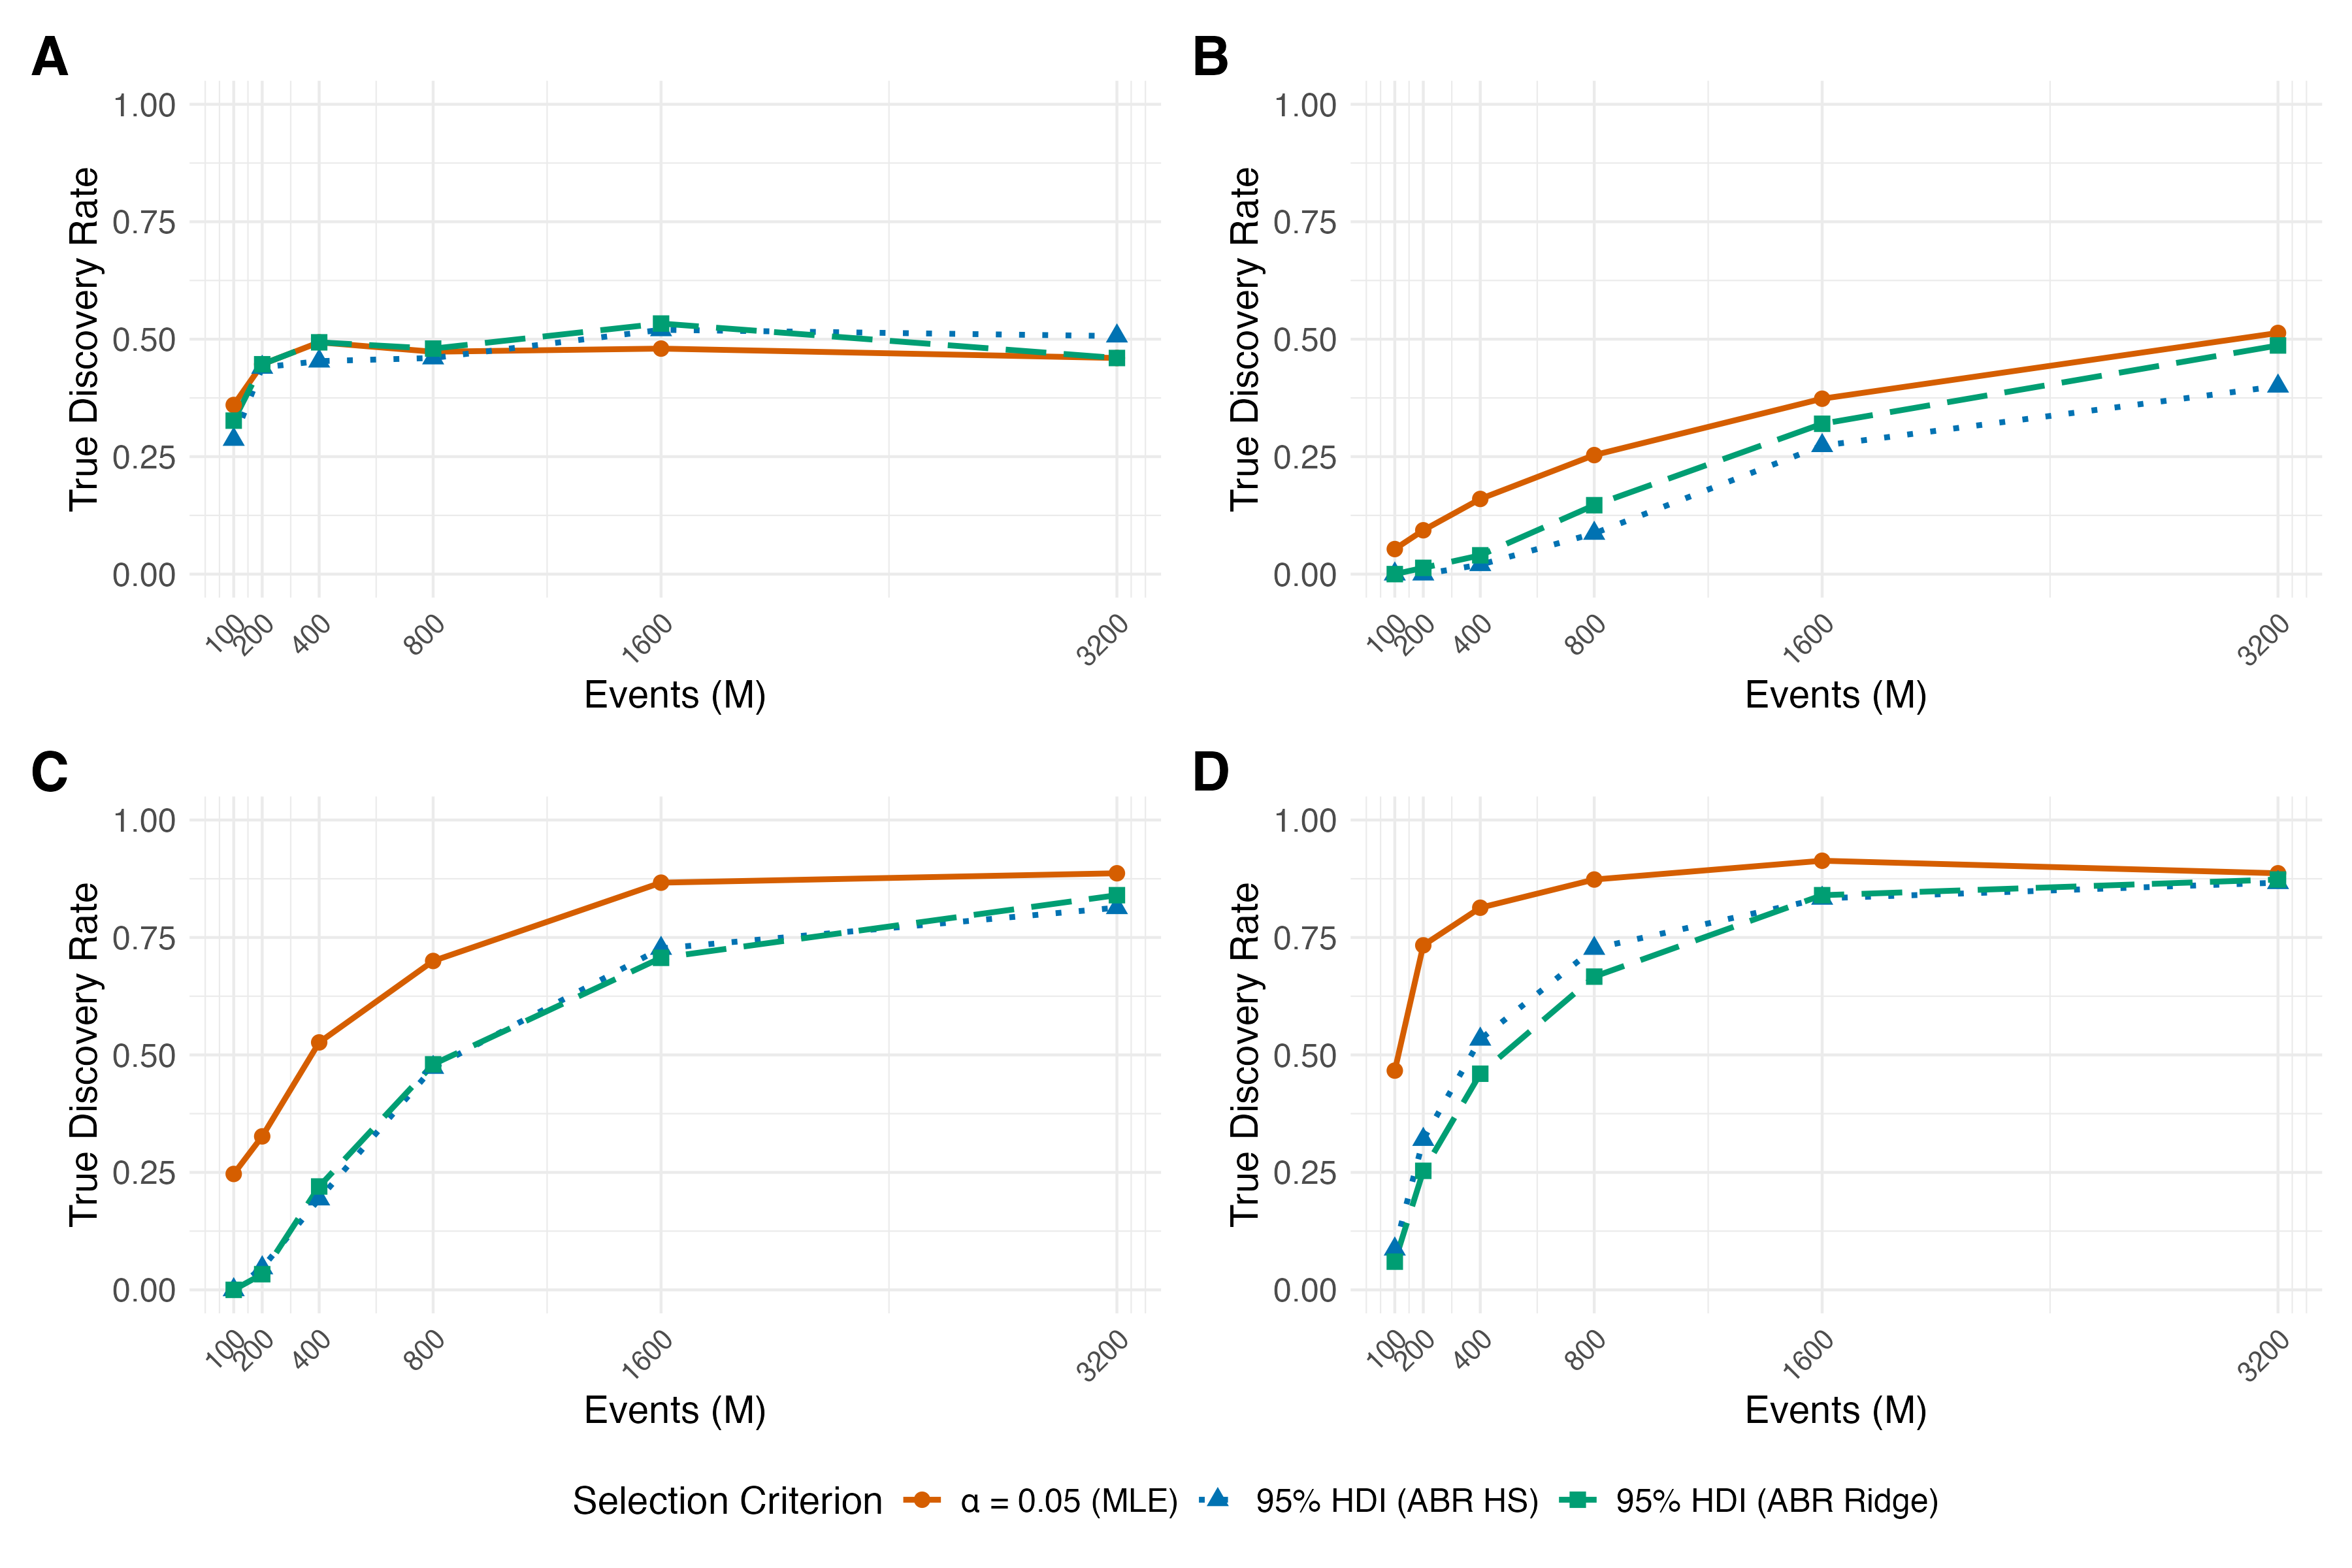
\includegraphics[width=\textwidth]{img/true_discovery_rates.png}
    \caption{True discovery rates (TDR) under varying effect sizes and numbers of events $M$ for endogenous and exogenous variables. Panels~(A)--(D) correspond to four scenarios: (A)~Endogenous Effects, (B)~Weak Exogenous Effects, (C)~Medium Exogenous Effects, and (D)~Strong Exogenous Effects. Horizontal axes show the number of events $M$ from 100 to 3200. Vertical axes represent the proportion of truly nonzero effects that are correctly identified (TDR). Three methods are compared: Maximum Likelihood Estimation (MLE) using univariate selection at $\alpha=0.05$ (solid orange line), Approximate Bayesian Regularization (ABR) with a Horseshoe prior applying the 95\% highest density interval (HDI) criterion (dotted blue line), and ABR with a Ridge prior applying the 95\% HDI criterion (long-dashed green line).}
    \label{fig:true_discovery_rates}
\end{figure}

Figure \ref{fig:true_discovery_rates} visualizes the true discovery rates over the 50 generated datasets by the number of events $M$ for the three endogenous effects, and the exogenous effects by effect size. MLE using univariate selection at $\alpha=0.05$ is generally most successful at selecting variables with truly nonzero effects. This advantage is strongest for exogenous effects of medium or strong effect sizes, particularly for smaller $M$s. Both criteria resulting from ABR  lead to lower true discovery rates. This can be explained by the addition of shrinkage, adding more probability mass in the posterior distribution near estimates of zero, thus leading to more HDIs that include zero. Somewhat surprising is the ability of the two ABR approaches to achieve a true discovery rate for endogenous effects that is comparable to - or for some $M$ even better than - the MLE model. Additionally, the selection criteria applied on the ABR models perform equally well for exogenous effects with higher $M$s, i.e. with $M=1600$ and $M=3200$. Between the two approaches utilizing ABR estimates, the model with the horseshoe prior performs better for all but weak exogenous effects. A likely explanation for this are the heavier tails of the horseshoe prior compared to the Normal Ridge prior. 

\begin{figure}[H]
    \centering
    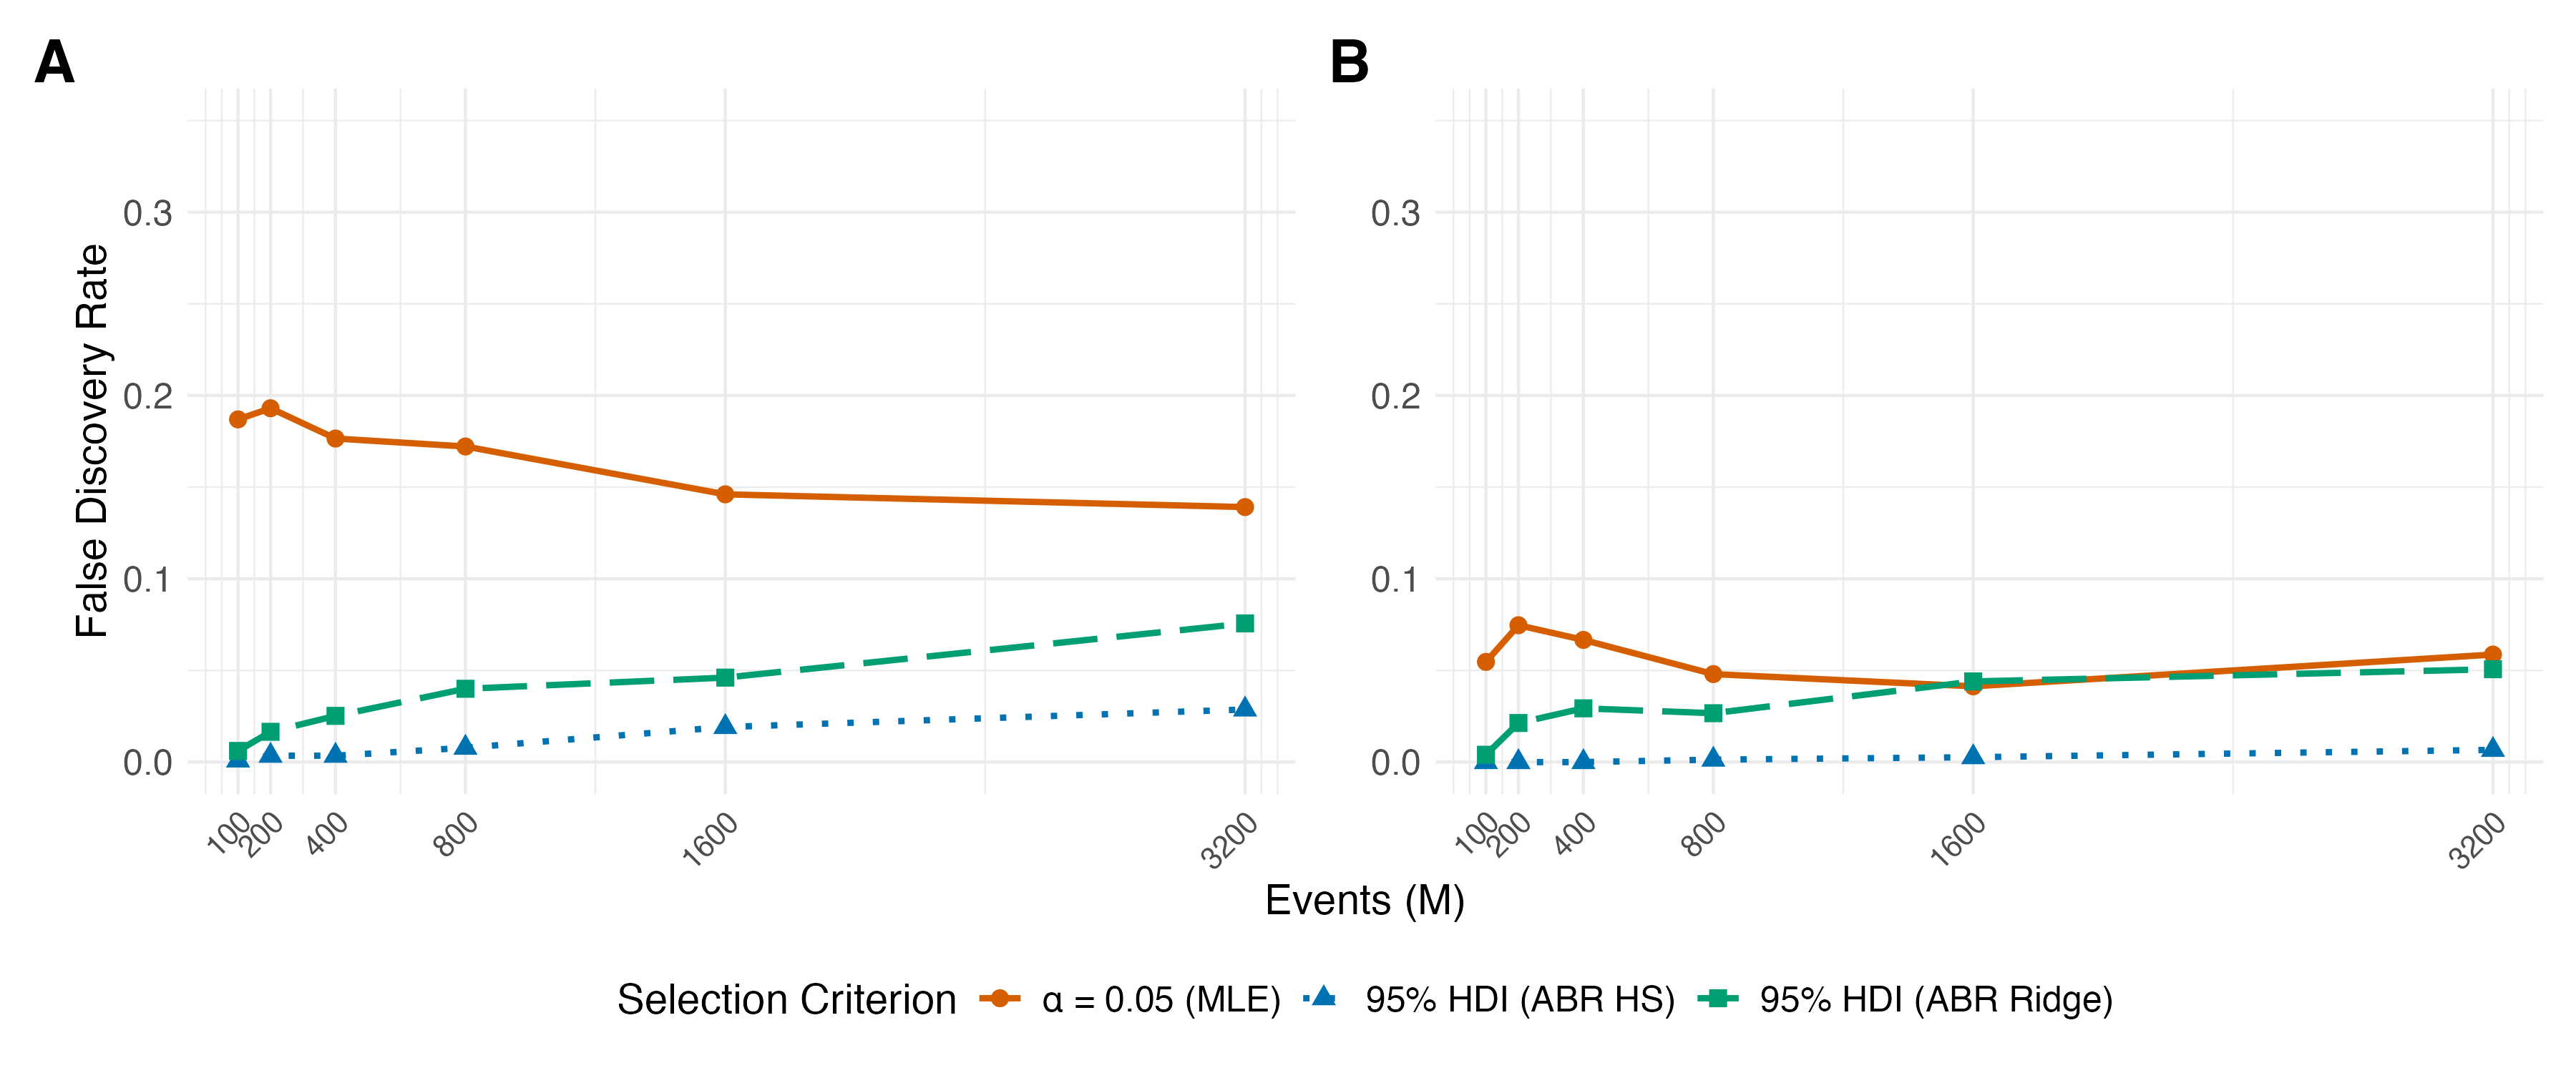
\includegraphics[width=\textwidth]{img/false_discovery_rates.png}
    \caption{False discovery rates (FDR) under varying numbers of events $M$ for endogenous and exogenous variables. Panels~(A) and (B) show two scenarios: (A)~Endogenous Effects, and (B)~Exogenous Effects. Horizontal axes display the number of events $M$ from 100 to 3200. Vertical axes represent the proportion of truly zero effects that are incorrectly identified as nonzero (FDR). Three methods are compared: Maximum Likelihood Estimation (MLE) using univariate selection at $\alpha=0.05$ (solid orange line), Approximate Bayesian Regularization (ABR) with a Horseshoe prior applying the 95\% highest density interval (HDI) criterion (dotted blue line), and ABR with a Ridge prior applying the 95\% HDI criterion (long-dashed green line).}
    \label{fig:false_discovery_rates}
\end{figure}

Figure \ref{fig:false_discovery_rates} displays the performance of the three selection criteria regarding false discovery rates for endogenous and exogenous effects by the number of events $M$. Similar to the true discovery rates, univariate selection with $\alpha=0.05$ leads to the highest rates of false discoveries. With type-I errors controlled at $\alpha=0.05$, the false discovery rates for exogenous effects align with expectations, being around 0.05 across all $M$s. In contrast, the higher rates for endogenous effects are surprising and a cause for concern. A plausible explanation may be high collinearity between endogenous statistics. By contrast, both penalization approaches perform better. Particularly, those resulting from shrinkage with a horseshoe prior perform best with false discovery rates particularly low for small $M$s.

Overall, estimates from all models show moderate levels of bias, with $\text{Bias}(\hat{\beta}_{\text{MLE}})=0.05$ being highest, and ABR models being lower ($\text{Bias}(\hat{\beta}_{\text{ABR}_{\text{HS}}})=0.01$; $\text{Bias}(\hat{\beta}_{\text{ABR}_{\text{Ridge}}})=-0.02$). This result is unexpected, as MLE is generally known to produce unbiased estimates \citep{Butts2008, Brandenberger2019}, but may stem from random variability caused by the relatively low number of generated datasets. An inspection of the estimates' variance demonstrates the instability of MLE estimates for low numbers of events $M$ (e.g., $\text{Var}(\hat{\beta}_{\text{MLE}}) = 3.16$ for $M=100$). Conversely, both ABR models yield estimates with lower variances.

Regarding predictive performance, the REMs from MLE generally perform best for in-sample predictions, as shown in Figure \ref{fig:predictive_performance}. This is to be expected, as they are specifically optimized to fit the observed data as closely as possible, minimizing the in-sample error. Compared to that, the REMs from ABR perform slightly worse, approaching MLE's performance as $M$ increases, potentially caused by the approximation's dependence on the error covariance matrix $\hat{\Sigma}_{\beta}$.

For out-of-samples, the ABR with a Ridge prior mostly performs similar or better than MLE, demonstrating the usefulness of regularization in avoiding overfitting. Particularly for smaller $M$s it is slightly superior to the REM from MLE. As $M$ increases, this advantage vanishes. Compared to that, ABR with a Horseshoe prior performs considerably worse.

\begin{figure}[H]
    \centering
    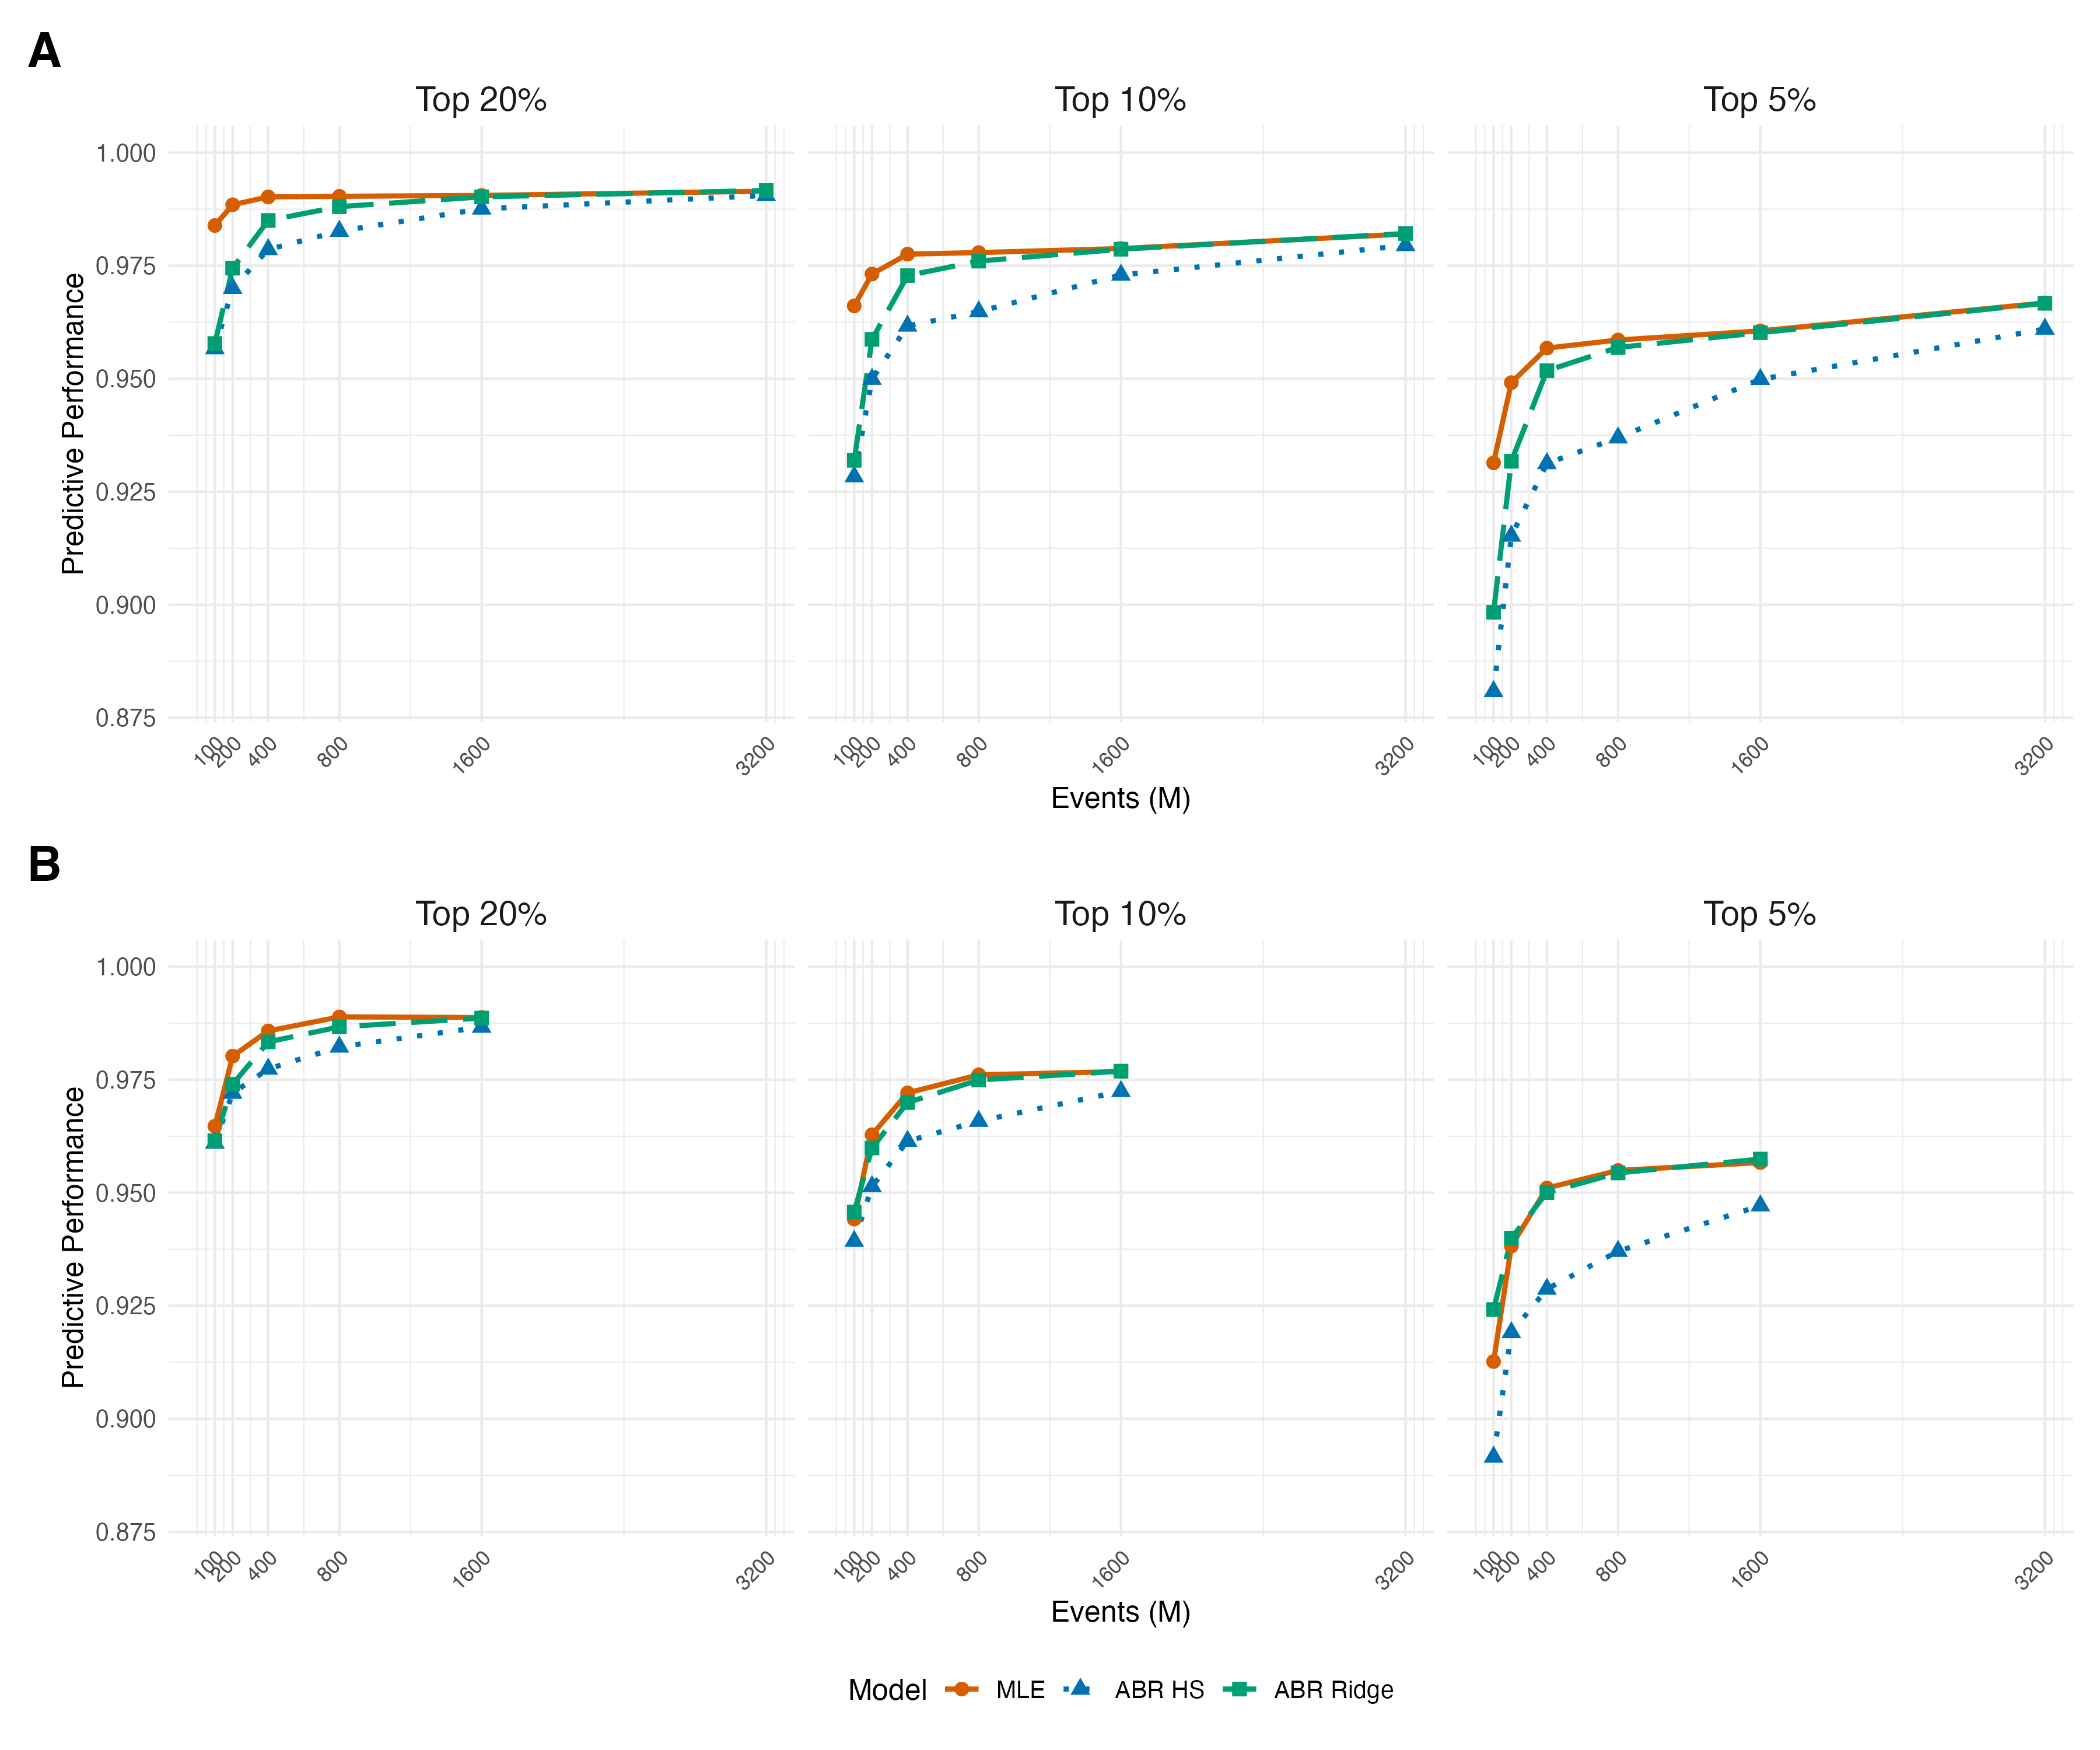
\includegraphics[width=\textwidth]{img/predictive_performance.png}
    \caption{Predictive performance assessed as the proportion of observed events ranking among the top 20\%, 10\%, and 5\% most probable events under three modeling approaches. Panel~(A) shows in-sample results; Panel~(B) shows out-of-sample results. Horizontal axes display the number of events $M$ from 100 to 3200, and vertical axes represent the proportion of observed events in the specified top-percentiles. Models include Maximum Likelihood Estimation (MLE, solid orange line), Approximate Bayesian Regularization with a Horseshoe prior (ABR HS, dotted blue line), and with a Ridge prior (ABR Ridge, long-dashed green line).}
    \label{fig:predictive_performance}
\end{figure}

\section{Discussion}

This report aimed at evaluating the performance of Approximate Bayesian Regularization (ABR) at variable selection and prediction in Relational Event Models (REMs) by comparing it to an approach utilizing maximum likelihood estimation (MLE). A simulation study was conducted where 50 relational event history (REH) datasets of $M=3200$ rows were generated and subsetted to different sizes to assess the behavior of three approaches across differently sized event lists. Regarding the selection of true effects, univariate selection using MLE estimates at $\alpha=0.05$ performed best, possessing the highest true discovery rate across most effect types and sizes. Regarding false discoveries, univariate selection, in turn, led to the highest rates. The procedure that best balanced true and false discovery rates was ABR with a horseshoe prior using the 95\% highest density interval criterion. Overall, the regularized coefficients exhibited the least bias, which may, however, be attributed to the relatively small number of datasets. Regarding predictive performance, REMs from MLE and ABR with a Ridge prior performed best for both in-sample and out-of-sample data.

What is missing here, is the exploration of alternative selection criteria in regularized models, beyond the 95\% HDI. This includes selecting variables with absolute effects exceeding specified thresholds. Additionally, considering recent works \citep{Amati2024, Boschi2024}, alternative metrics for assessing predictive performance should be explored, given that the current method overlooks the role of time points $t$ in coefficient estimation.

As regularization is particularly superior to MLE in high-dimensional settings (i.e., where the ratio of observations to predictors is low), an increased number of potential actors could be examined, as MLE demonstrates lower statistical power with larger risksets \citep{Schecter2020}. Moreover, examining the inclusion of interaction effects between endogenous and exogenous variables, which would further increase dimensionality, remains to be explored. In light of the observed bias in MLE estimates, more datasets need to be generated.

Therefore, the thesis project will focus on assessing Bayesian regularization performance in higher dimensionality through simulations using additional generated datasets. In doing so, exact Bayesian regularization will be compared to the approximation presented here, with REMs being rewritten to Poisson regression models \citep{Vieira2024}.

In conclusion, this report provides indications of the advantages of approximate Bayesian regularization for variable selection and prediction in Relational Event Models, but further more extensive evaluations are needed to obtain more reliable results.


\end{justify}
\end{spacing}

\newpage

\bibliographystyle{apalike}
\bibliography{literature.bib}

\end{document}